\documentclass{article}
\usepackage{graphicx}
\usepackage[margin=1.5cm]{geometry}
\usepackage{amsmath}

\begin{document}

\title{Thursday Reading Assessment: Chapter 6}
\author{Prof. Jordan C. Hanson}

\maketitle

\begin{figure}[ht]
\centering
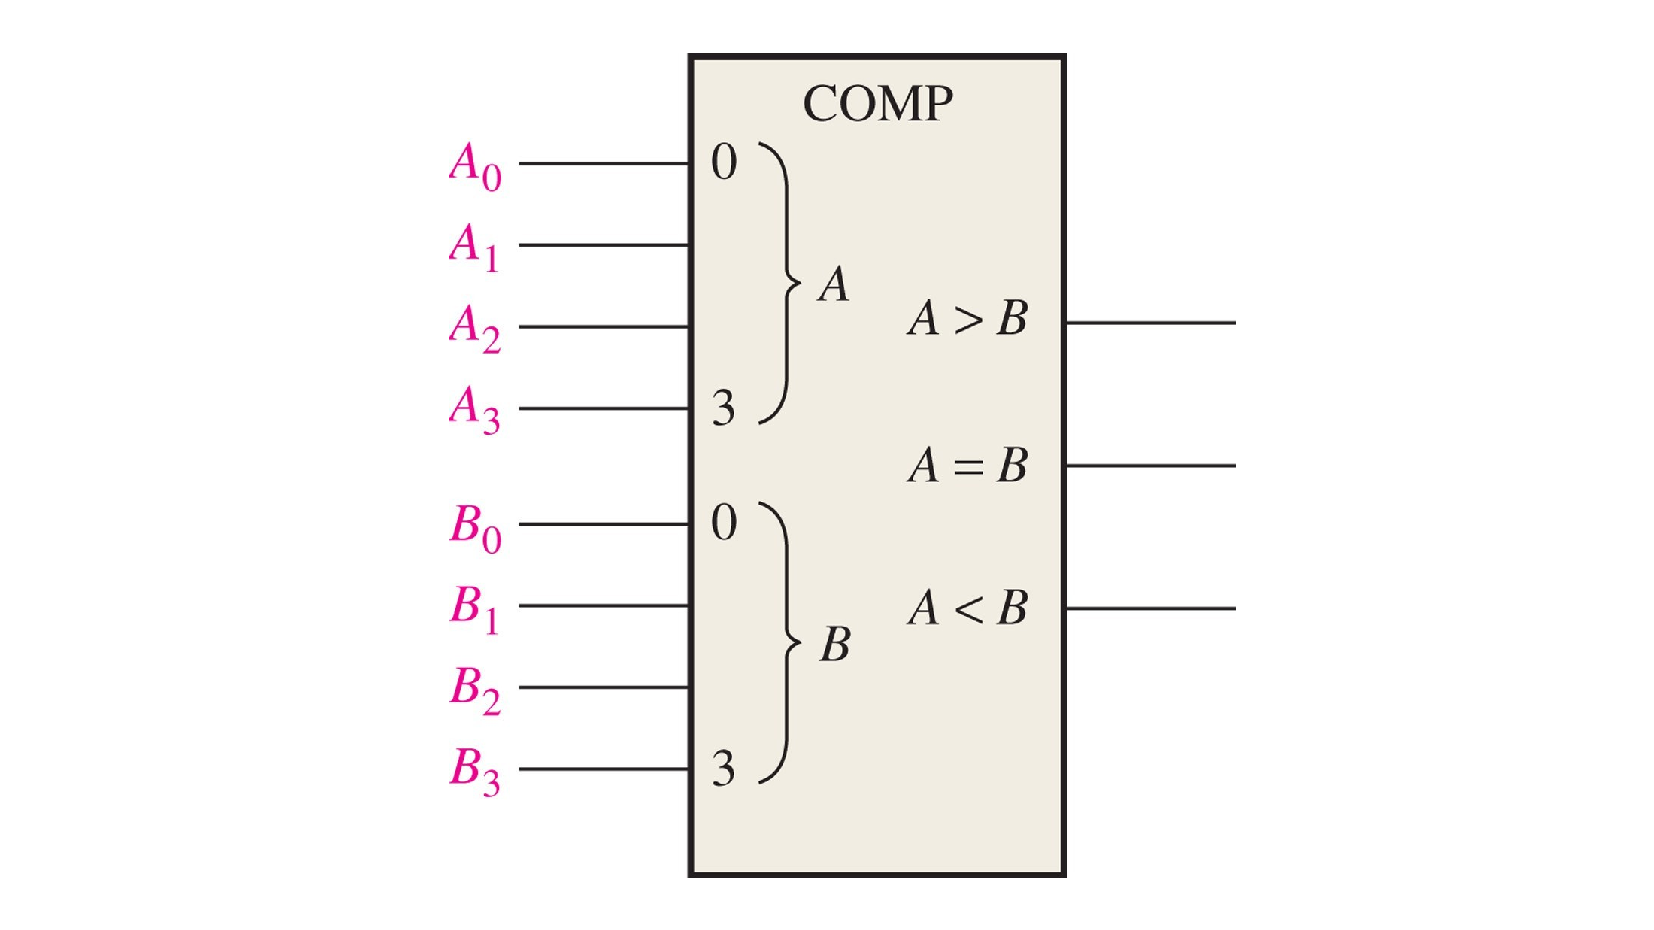
\includegraphics[width=0.33\textwidth]{figures/comparator3.pdf} \hspace{0.5cm}
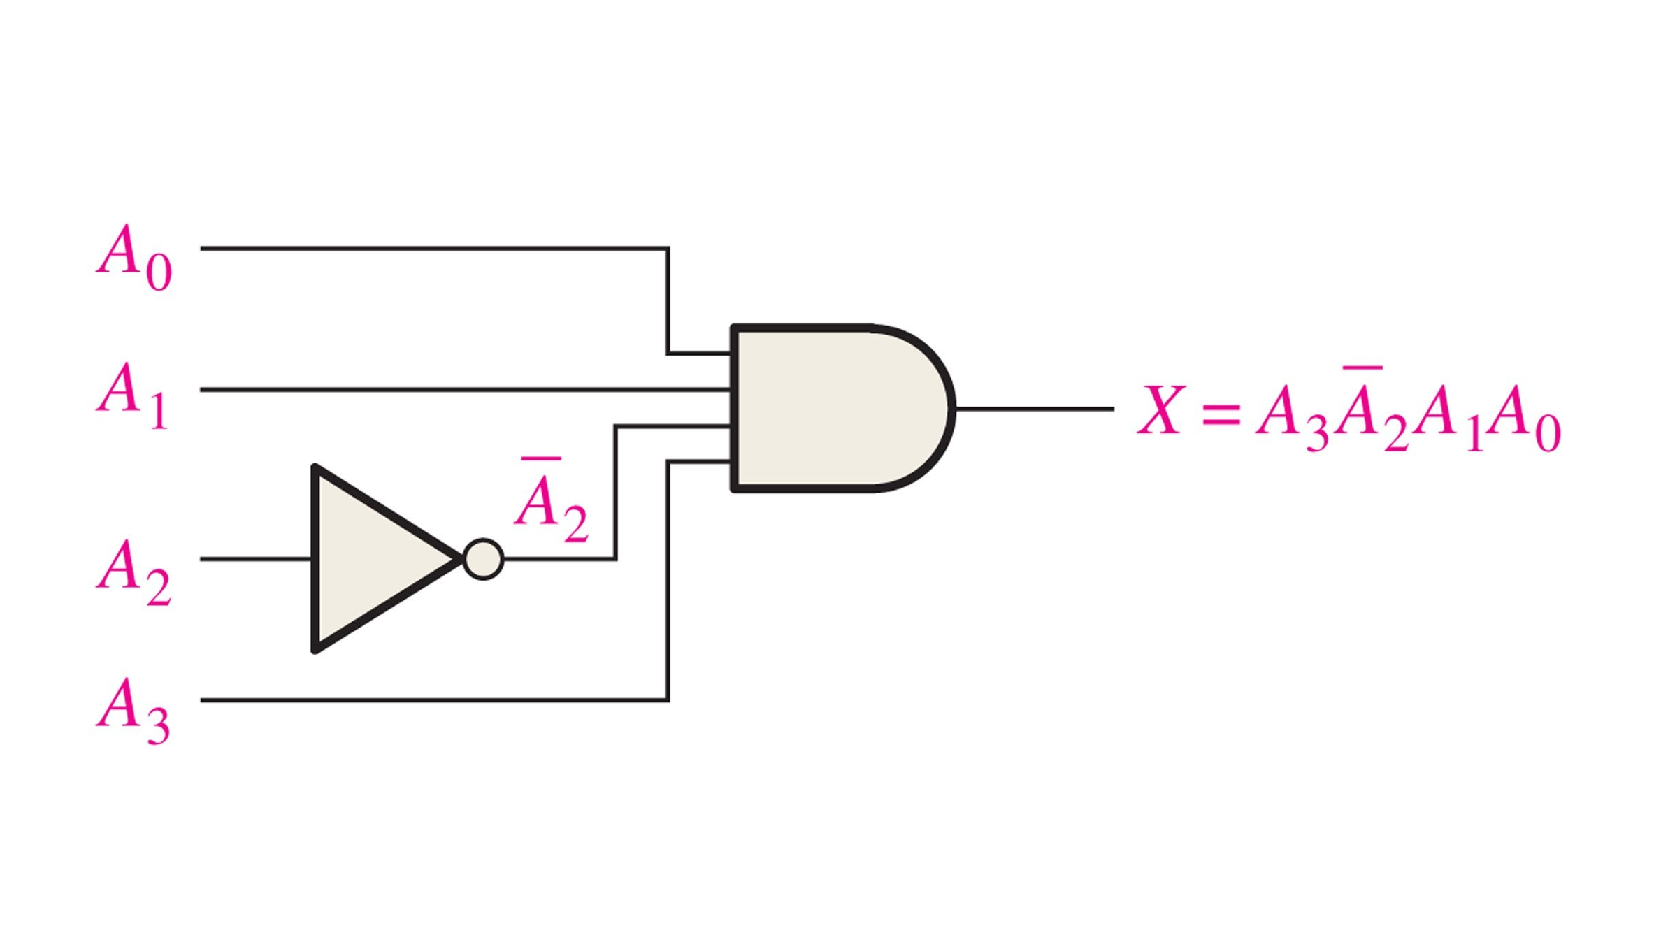
\includegraphics[width=0.33\textwidth]{figures/decoder2.pdf}
\caption{\label{fig:1} (Left): A comparator for two 4-bit numbers. (Right) A decoding function for the code 1011.}
\end{figure}

\section{Functions of Combinational Logic: Comparators}

\begin{enumerate}
\item (a) Assess the \textit{power consumption} of the component in Fig. \ref{fig:1} (left).  Assume that each XOR and AND gate consumes $\approx 100$ $\mu$W per gate.  Recall the gates that make a 1-bit comparator.  Perform the calculation for just the equality function, assuming the $A>B$ and $A<B$ functions are not connected.  (b) \textbf{Bonus point:} Try the calculation for $A>B$ and $A<B$, assuming 100 $\mu$W/gate.  \\ \vspace{3cm}
\end{enumerate}

\section{Functions of Combinational Logic: Decoders}

\begin{enumerate}
\item Consider Fig. \ref{fig:1} (right), in which the decoding function for 1011 is displayed.  Generate all gate diagrams for the BCD codes.  That is, for codes 0000, 0001, ... generate circuits that go HIGH to represent the digits 0-9. \\ \vspace{5cm}
\end{enumerate}

\end{document}
